\section{Integer programs and relaxation: the good, the bad, and the ugly}
\label{sec-ilp}

\noindent 
In the previous parts we showed how the linear programming problem can be solved efficiently.
In solving real-life problems, we are often interested only in solutions where some of the 
variables involved are forced to be integers. In the first motivation example we found out
that the optimal solution is to buy $2\frac{2}{3}$ dl of green stuff. This would probably not
be feasible, since drinks are usually served in multiples of some fixed volume. 


\begin{center}
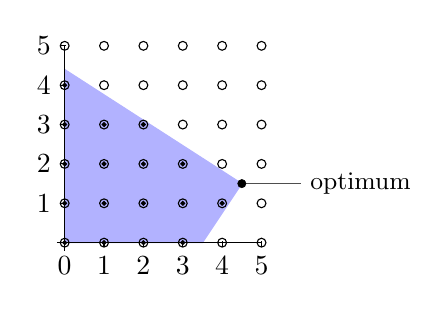
\begin{tikzpicture}[scale=0.5]

  \filldraw[color=blue!30]
  (0,0) -- (3.5,0) -- (4.5,1.5) -- (0,4.4) -- cycle;

  \halfplane{0,0}{5,0}{+}{0.5cm}{0.8cm}
  \halfplane{3.5,0}{4.5,1.5}{+}{0.2cm}{2.4cm}
  \halfplane{0,4.4}{4.5,1.5}{-}{0.5cm}{2.4cm}
  \halfplane{0,0}{0,5}{-}{0.5cm}{1cm}

  %\draw 
  %  (0,3.5) node[anchor=south west]{$x\ge 0$}
  %  (2,3.5) node[anchor=south west]{$x\le 2$}
  %  (2.5,1.8) node[anchor=south west]{$x\ge y$}
  %  (2.5,0.3) node[anchor=south west] {$y\ge 0$};


  \draw
    \foreach \x in {0,...,5}
      \foreach \y in {0,...,5}
      {(\x,\y) circle (3.2pt)};

  \filldraw
  \foreach \x in {0,...,2}
      \foreach \y in {0,...,2}
      {(\x,\y) circle (1.4pt)};
  
  \filldraw   
  \foreach \p in {(0,3),(0,4),(1,3),(3,2),(3,1),(4,1),(2,3),(3,0)}
      {\p circle (1.4pt)};

  %axis
  \draw (-.2,0) -- coordinate (x axis mid) (5,0);
  \draw (0,-.2) -- coordinate (y axis mid) (0,5);
  %ticks
  \foreach \x in {-0,...,5}
      \draw (\x,1pt) -- (\x,-3pt);
  \foreach \x in {0,...,5}
      \draw (\x,-3pt) node[anchor=north] {\x};
  \foreach \y in {1,...,5}
      \draw (1pt,\y) -- (-3pt,\y)
          node[anchor=east] {\y};

  \filldraw[very thin]
    (4.5,1.5) circle (3pt)
    (6,1.5) -- (4.5,1.5)
    (6,1.5) node[anchor=west] {{\small optimum}};

    
\end{tikzpicture}
\mycaption{Feasible solutions of a linear program and its integral restriction.}
\end{center}

\noindent 
The first intuition might suggest that this is just a small technical issue: after all, we can always find the 
optimal solution of the continuous version, round it in some way and get, if not the optimal solution, then 
surely something reasonably close to the optimum. On a second thought one starts wondering that it might not be
so easy: if a linear program  used to find out whether to travel by air or by train
recommends to buy half air and half train ticket, the rounding is as complex as the entire solution. The following 
picture shows that the closest integer solution might be quite far from the optimum, and it is not obvious how to
find it. 

\begin{center}
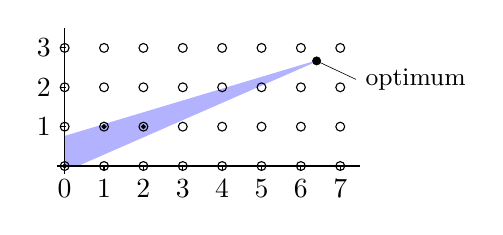
\begin{tikzpicture}[scale=0.5]

  \filldraw[color=blue!30]
  (0,0) -- (0.3,0) -- (6.4,2.67) -- (0,0.75) -- cycle;

  \halfplane{0,0}{7,0}{+}{0.5cm}{0.8cm}
  \halfplane{0.3,0}{6.4,2.67}{+}{0.2cm}{2.4cm}
  \halfplane{0,0.75}{6.4,2.67}{-}{0.5cm}{2.4cm}
  \halfplane{0,0}{0,3}{-}{0.5cm}{1cm}



  \draw
    \foreach \x in {0,...,7}
      \foreach \y in {0,...,3}
      {(\x,\y) circle (3.2pt)};

  \filldraw   
  \foreach \p in {(0,0),(1,1),(2,1)}
      {\p circle (1.4pt)};

  %axis
  \draw (-.2,0) -- coordinate (x axis mid) (7.5,0);
  \draw (0,-.2) -- coordinate (y axis mid) (0,3.5);
  %ticks
  \foreach \x in {-0,...,7}
      \draw (\x,1pt) -- (\x,-3pt);
  \foreach \x in {0,...,7}
      \draw (\x,-3pt) node[anchor=north] {\x};
  \foreach \y in {1,...,3}
      \draw (1pt,\y) -- (-3pt,\y)
          node[anchor=east] {\y};

  \filldraw[very thin]
    (6.4,2.67) circle (3pt)
    (7.4,2.2) -- (6.4,2.67)
    (7.4,2.2) node[anchor=west] {{\small optimum}};

\end{tikzpicture}
\end{center}

\noindent 
A linear program with some variables constrained to be integers is called an integral linear program (ILP):


\begin{framed}
  \begin{dfn}
    {\em An integral  linear program} (ILP) in a normal form is a linear program 
    $$ \max_{\bm{x}\in\R^n}\left\{ \bm{c}\tr\bm{x} \mid A\bm{x}=\bm{b},\;\bm{x}\ge\bm{0}\right\}$$
    with additional constraints of the form $x_i\in\Z$.
  \end{dfn}
\end{framed}

\noindent 
A reader with some background in the complexity theory is surely not surprised by the fact that the integrality
constraints significantly increase the expressive power of linear programs. When formulating problems in terms of 
linear programs important role is played by so called {\em indicator variables}: a set of variables  $\delta_1,\ldots,\delta_k\in\Z$ 
with constraints 
\begin{align*}
  \delta_1+\delta_2+\cdots+\delta_k&=1\\
  \delta_i&\ge0\text{\ pre\ }i=1\ldots k
\end{align*}
have the property that in any feasible solution is exactly one $\delta_i=1$, and the rest of them is zero.
Indicator variables allow to express the selection of one alternative among several possibilities, and
thus e.g. describe complex non-convex domains. As a demonstration, let us suppose that we want to maximize the 
function $f(x,y)=x+y$ over the following domain \dom:

\begin{myfig}{0.4\textwidth}{svg/nekonvex-a}
\end{myfig}

\noindent
The domain \dom can be decomposed into 5 parts:
\begin{myfig}{0.4\textwidth}{svg/nekonvex}
\end{myfig}
such that each of them can be represented by linear constraints:
\begin{align*}
  x&\ge0    & x&\ge1 & x&\ge1 & x&\ge2    & x&\ge4\\
  x&\le1    & x&\le2 & x&\le2 & x&\le3    & x&\le5\\
  y&\ge1-x  & y&\ge2 & y&\ge0 & y&\ge x-2 & y&\le6x-24\\
  y&\le2+x  & y&\le3 & y&\le1 & y&\le5-x  & y&\le-6x+30\\
   &        &  &     &  &     &  &        & y&\ge0
\end{align*}
Let us introduce indicator variables
$\delta_1,\ldots,\delta_5\in\Z$ 
and rewrite each set of constraints describing one part, such that if the corresponding indicator is zero they
yield trivial constraints, and if the indicator is one they retain their original values. In this way we obtain 
an ILP: the task is to maximize $x+y$, subject to the constraints:


\begin{align*}
  x&\ge0                  & x&\ge\delta_2    & x&\ge\delta_3    & x&\ge2\delta_4            & x&\ge4\delta_5\\
  x&\le5-4\delta_1        & x&\le5-3\delta_2 & x&\le5-3\delta_3 & x&\le5-2\delta_4          & x&\le5\\
  y&\ge\delta_1-x         & y&\ge2\delta_2   & y&\ge0           & y&\ge-5+3\delta_4+x  & y&\le3-27\delta_5+6x\\
  y&\le3-\delta_1+x   & y&\le3           & y&\le3-4\delta_3 & y&\le8-3\delta_4-x    & y&\le33-3\delta_5-6x\\
   &                      &  &               &  &               &  &                        & y&\ge0
\end{align*}

\noindent 
Another useful property of integer programs is the possibility to approximate the optimization of non-linear
utility functions by piecewise-linear functions. Let us suppose that, in the previous example, instead of 
maximizing the function $x+y$, we want to maximize the function composed of linear pieces:
\begin{myfig}{0.55\textwidth}{svg/nonlinear-a}
\end{myfig}

\noindent 
Let us introduce four variables $z_1,z_2,z_2,z_3,z_4$ that 
denote to what extent is the corresponding interval covered by the amount $x+y$:
$$x+y=z_1+z_2+z_3+z_4$$
We need some additional constraints that ensure that the $z_i$s will be ``filled consecutively'',
i.e. if $z_i$ is non-zero then $z_{i-1}$ is at its maximum. 

\noindent
\begin{minipage}[t]{0.5\textwidth}
  \vskip 0pt
\begin{myfig}{\textwidth}{svg/nonlinear}
\end{myfig}
\end{minipage}
\hspace*{1cm}
\begin{minipage}[t]{0.5\textwidth-1cm}
\vskip 0pt
In order to do so, we add three binary variables
$\alpha_1,\alpha_2,\alpha_3$,
where $\alpha_i\in\Z$, $0\le\alpha_i\le1$
with the meaning that that the variable $\alpha_i\in\{0,1\}$ indicates whether  $z_{i+1}$ 
is non-zero. The constraints:
\begin{align*}
  2\alpha_1&\le z_1\le2\\
  \alpha_2&\le z_2\le\alpha_1\\
  2\alpha_3&\le z_3\le2\alpha_2\\
  0&\le z_4\le3\alpha_3
\end{align*}
then ensure the required properties, e.g. if $\alpha_1=0$, then  $0\le z_1\le2$, but $z_2=z_3=z_4=0$.
On the other hand, if  $\alpha_1=1$, then  $z_1=2$ and $\alpha_2\le z_2\le1$.
Using these variables, the utility function is easily expressed as
\end{minipage}

$$f(x,y,z_1,\ldots,z_4,\alpha_1,\ldots,\alpha_3,\delta_1,\ldots,\delta_5)=1+\frac{1}{2}z_1+4z_2-2z_3-\frac{1}{2}z_4$$


\vskip 1ex \noindent 
The previous examples have hopefully supported the reader's intuition that ILP can express much 
more complicated problems than LP, and so the solution of the ILP should be harder than that of LP.
We show that it is indeed so: even the problem of determining whether there is any feasible solution
 to a given ILP is \NP-complete (and so the author of this text does not expect a polynomial time-algorithm
for solving the ILP will be found). For our proof, we shall need the \sat problem, so let's review its
definition:

\begin{framed}
  \begin{dfn}
    \label{dfn:sat}
    Given $n$ logical variables $x_1,\ldots,x_n\in\{true,false\}$, a {\em literal}
    is either a variable $x_i$ or its negation $\neg{x_i}$, a {\em clause} is 
    a disjunction of literals $C=l_1\vee l_2\vee\cdots\vee l_{k_C}$, and a formula
    in a conjunctive normal form (CNF) is a conjunction of clauses
    $F=C_1\wedge C_2\wedge\cdots\wedge C_m$. The problem \sat is a decision 
    problem where for a given CNF formula $F$, the task is to decide whether there exists a
    satisfying truth assignment, i.e. an assignment of values $\{true, false\}$ to variables
    $x_1,\ldots,x_n$ such that $F$ is true.
  \end{dfn}
\end{framed}

\noindent 
A fundamental result in the complexity theory is the Cook-Lewin theorem stating that \sat is \NP-complete,
i.e. the existence of a polynomial-time algorithm for \sat would imply $\P=\NP$.
Now we show that if there would exist a polynomial-time algorithm \algA deciding, for any ILP, whether there 
exists some feasible solution, there would be a polynomial-time algorithm \algA' solving \sat. Let us suppose we
have given the algorithm \algA, and we shall describe the algorithm \algA'. Let the input formula $F$ consits of 
clauses   $C_1,\ldots,C_m$. Denote by  $P_i$ the set of variables that appear in $C_i$ as positive literals, and
$N_i$ the set of variables those variables that appear in $C_i$ in negated literals. E.g. for the clause 
$C_i=(x_1\vee\neg{x_2}\vee x_3)$ we have $P_i=\{x_1,x_3\}$ and
$N_i=\{x_2\}$.  Construct an ILP $I$ such that to each logical variable $x_i$ there will be an equally denoted
variable $x_i\in\Z$ constrained to $0\le x_i\le1$. 
In a satisfying truth assignment, at least one literal must be true in any clause $C_i$, which can be expressed
as a constraint
$$\sum_{x\in P_i}x + \sum_{x\in N_i}(1-x) \ge 1$$
For example, for the formula
$$(x_1\vee x_2\vee x_3)\wedge(\neg{x_1}\vee\neg{x_2}\vee\neg{x_3})\wedge(x_1\vee\neg{x_2}\vee\neg{x_3})\wedge(\neg{x_1}\vee\neg{x_2}\vee x_3)\wedge(\neg{x_1}\vee x_2\vee x_3)$$
we get constraints
\begin{align*}
  x_1+x_2+x_3&\ge1\\
  (1-x_1)+(1-x_2)+(1-x_3)&\ge1\\
  x_1+(1-x_2)+(1-x_3)&\ge1\\
  (1-x_1)+(1-x_2)+x_3&\ge1\\
  (1-x_1)+x_2+x_3&\ge1\\
  x_1,x_2,x_3&\ge0\\
  x_1,x_2,x_3&\le1
\end{align*}
Clearly any satisfying assignment $F$ is a feasible solution of $I$, and vice versa. Hence, the formula $F$ is 
satisfiable if and only if there exists a feasible solution of $I$.

\begin{prob}
  Try to express other \NP-hard problems (e.g. the Traveling Salesman Problem, Maximum Clique Problem, \ldots)
  as ILP.
\end{prob}

\vskip 1ex \noindent 
Our previous thoughts can be summarized as follows: ILP is a general framework that can  express many
optimization problems. This expressive power, however, comes at a cost, since we don't expect a
polynomial-time algorithm for solving ILP to exist.

\subsection*{The good: \maxWBmatching}

Imagine you are writing a program to play a turn-based strategic game. In a turn, several
units can be activated: each of them can move next to some enemy unit, and potentially attack it.
After an attack, the figure is not allowed to  move anymore, and since any tile can be occupied
by at most one unit, no two units cannot attack from the same tile. Every potential attack 
has a known damage, and the task is to move the units in such a way that maximizes the overall 
damage.\footnote{Admittedly, this is not the best possible overall strategy, but the 
task may be used as a subproblem in some specific cases.}


\begin{myfig}{0.8\textwidth}{svg/match}
  Each unit in the bottom line can be moved to some of the indicated blue tiles and attack an enemy unit.
  The numbers represent the damage dealt by the corresponding attack. The optimal attack is highlighted.
\end{myfig}


\noindent
The problem we are facing is known as the Maximum Bipartite Matching problem\footnote{%
This problem is somewhat special: most of the problems presented in this course are \NP-hard, but
\maxWBmatching is not. The reader may be familiar with an efficient algorithm to solve this problem.
Even if it is the case, we ask the reader to follow our exposition, as it is meant to give an insight 
into the properties of ILPs.}:


\begin{framed}
  \begin{dfn}
    \label{dfn:maxWBmatching}
    Given a bipartite graph with edges labeled by non-negative weights, the \maxWBmatching
    problem asks to select a set of edges with maximal overall weight in such a way that no
    two selected edges share a common vertex.
  \end{dfn}
\end{framed}

\noindent The problem \maxWBmatching 
can be formulated as an ILP problem: given a bipartite graph $G=(V,E)$ with edge-weights
$\omega:E\mapsto\R^+$, let us introduce a selector variable  $x_e\in\{0,1\}$ for each edge $e\in E$,
that is selected if the corresponding edge has been included in the matching. The goal is to maximize the sum
of the weights of the selected edges, i.e. 
$\max\sum_{e\in E}\omega_ex_e$
What remains is to design a set of linear constraints that ensure that the selected edges form a matching.
The whole ILP then looks as follows (the constrains $x_e\le1$ don't have to be written explicitly, since
they are implied by the rest of the program):

\begin{equation}
\label{eq:ILPa:1}
\begin{array}{rrcll}
  {\rm maximize}     & \multicolumn{1}{l}{\sum\limits_{e\in E}\omega_ex_e}\\[3ex]
  {\rm subject\ to} & \sum\limits_{e\in E\atop e=(v,w)}x_e&\le&1& \;\;\;\forall v\in V\\
                          & x_e&\ge&0& \;\;\;\forall e\in E\\
                          & x_e&\in&\Z
\end{array}
\end{equation}

\noindent
For example, for the graph on the left we get the constraints\\
\begin{minipage}[t]{0.4\textwidth}
  \vskip 0pt
  \begin{myfig}{0.8\textwidth}{svg/match-2}
\end{myfig}
\end{minipage}
\begin{minipage}[t]{0.6\textwidth}
\vskip 0pt
\begin{align}
  x_{e_1}&\le1\notag\\
  x_{e_2}+x_{e_4}&\le1\notag\\
  x_{e_3}+x_{e_5}&\le1\notag\\
  x_{e_1}+x_{e_2}+x_{e_3}&\le1\label{eq:ILPa:2}\\
  x_{e_4}+x_{e_5}&\le1\notag\\
  x_{e_1},x_{e_2},x_{e_3},x_{e_4},x_{e_5}&\ge0\notag
  %x_{e_1},x_{e_2},\ldots,x_{e_5}&\in\Z\\
\end{align}
\end{minipage}

\noindent 
Since we have no efficient algorithm for solving ILP, we can try to solve the {\em relaxed } LP, where
the constraints $x_e\in\Z$ are left out of the program (\ref{eq:ILPa:1}).
Clearly, all the feasible solutions of the ILP are also feasible solutions of the relaxed program, so the 
optimum of the relaxed program is an upper bound on the optimum of the ILP. As we have already seen, solving 
the relaxed program is in general a bad idea, since the optimum of the ILP can be really far away from the optimum
of the relaxed program. However, we are not interested in arbitrary programs, but only in those that are obtained
the way we described from some bipartite graph. This gives us hope that maybe due to the inherent structure of these 
programs  some information about the solution of the ILP is contained in the optimal solution of the relaxed program.
For example, let us use the constraints from 
(\ref{eq:ILPa:2}), and let us set  $\omega_{e_1}=1$ and
$\omega_{e_2}=\cdots=\omega_{e_5}=10$. When we try to solve the relaxed linear program using the simplex
method\footnote{For increased dramatic effect we encourage the reader to really try it.}, to our pleasant 
surprise the found optimal solution will be integral, although there surely exist also non-integral optimal
solutions (e.g. $x_{e_1}=0$,
$x_{e_2}=\cdots=x_{e_5}=\frac{1}{2}$).
We can try different weights, and different graphs, and, surprisingly, the result is always the same:
the LP solver for the relaxation always finds an integral optimal solution. Let's investigate this strange behavior
further. We write our program in the matrix form
$$\max\{\bm{c}\tr\bm{x}\mid A\bm{x}\le\bm{b},\;\bm{x}\ge\bm{0}\}$$
where
\begin{align*}
\bm{c}&=\left(\begin{array}{c}1\\10\\10\\10\\10\end{array}\right)&
A&=\left(\begin{array}{ccccc}1&0&0&0&0\\0&1&0&1&0\\0&0&1&0&1\\1&1&1&0&0\\0&0&0&1&1\end{array}\right)&
\bm{x}&=\left(\begin{array}{c}x_{e_1}\\x_{e_2}\\x_{e_3}\\x_{e_4}\\x_{e_5}\end{array}\right)&
\bm{b}&=\left(\begin{array}{c}1\\1\\1\\1\\1\end{array}\right)
\end{align*}
The matrix  $A$ represents the bipartite graph in a way that there is one row for each vertex, and one column for
each edge. In each column, there are ones in the rows corresponding to the (two) vertices incident with the given 
edge. Such a matrix is called the {\em incidence matrix} of a bipartite graph. In our particular case, we can further
simplify the program by leaving the first row out: the constraint $x_{e_1}\le1$ is implied by 
$x_{e_1}+x_{e_2}+x_{e_3}\le1$, and the fact that the variables are non-negative.
We introduce the slackness variables, and obtain a linear program in the normal form:
\begin{equation}
  \label{eq:ILPa:3}
  \max\{\bm{\tilde{c}}\tr\bm{\tilde{x}}\mid \tilde{A}\bm{\tilde{x}}=\bm{\tilde{b}},\;\bm{\tilde{x}}\ge\bm{0}\}
\end{equation}
where
\begin{align*}
\bm{\tilde{c}}&=\left(\begin{array}{c}1\\10\\10\\10\\10\\0\\0\\0\\0\end{array}\right)&
\tilde{A}&=\left(\begin{array}{ccccccccc}0&1&0&1&0&1&0&0&0\\0&0&1&0&1&0&1&0&0\\1&1&1&0&0&0&0&1&0\\0&0&0&1&1&0&0&0&1\end{array}\right)&
\bm{\tilde{x}}&=\left(\begin{array}{c}x_{e_1}\\x_{e_2}\\x_{e_3}\\x_{e_4}\\x_{e_5}\\s_1\\s_2\\s_3\\s_4\end{array}\right)&
\bm{\tilde{b}}&=\left(\begin{array}{c}1\\1\\1\\1\end{array}\right)
\end{align*}

\noindent
Recall the definition of a basic solution. For each basis $B$, the matrix   $\tilde{A}_B$
is a non-singular square matrix of dimensions $4\times 4$; the non-basic variables are all zeroes, and the 
values of basic variables are given by the solution of the system 
$$\tilde{A}_B\bm{\tilde{x}}_B=\bm{\tilde{b}}.$$
Using the Cramer rule, the $i$-th component of the solution is given by
$$\frac{\det\left(\tilde{A}_B\langle i\rangle\right)}{\det\left(\tilde{A}_B\right)}$$
where $\tilde{A}_B\langle i\rangle$ is a matrix obtained from  $\tilde{A}_B$
by replacing the $i$-th column by the right-hand side vector $\bm{\tilde{b}}$.
For example, the basis $B=(2,4,7,8)$ yields a system
$$\tilde{A}_B\bm{\tilde{x}}_B=\left(\begin{array}{cccc}1&1&0&0\\0&0&1&0\\1&0&0&1\\0&1&0&0\end{array}\right)
\left(\begin{array}{c}x_{e_2}\\x_{e_4}\\s_2\\s_3\end{array}\right)=
\left(\begin{array}{c}1\\1\\1\\1\end{array}\right)
$$
The following determinants are needed to solve the system using the Cramer rule:
$$\det\left(\tilde{A}_B\right)=\left|\begin{array}{cccc}1&1&0&0\\0&0&1&0\\1&0&0&1\\0&1&0&0\end{array}\right|=1$$
\renewcommand{\tmp}{\bm{{\color{red}1}}}
\begin{align*}
\left|\begin{array}{cccc}\tmp&1&0&0\\\tmp&0&1&0\\\tmp&0&0&1\\\tmp&1&0&0\end{array}\right|&=0&
\left|\begin{array}{cccc}1&\tmp&0&0\\0&\tmp&1&0\\1&\tmp&0&1\\0&\tmp&0&0\end{array}\right|&=1&
\left|\begin{array}{cccc}1&1&\tmp&0\\0&0&\tmp&0\\1&0&\tmp&1\\0&1&\tmp&0\end{array}\right|&=1&
\left|\begin{array}{cccc}1&1&0&\tmp\\0&0&1&\tmp\\1&0&0&\tmp\\0&1&0&\tmp\end{array}\right|&=1
\end{align*}
We obtained a solution
  $x_{e_2}=0, x_{e_4}=1, s_2=1, s_4=1$
that can be interpreted as a (non optimal) matching where only the edge $e_4$ is selected; the
slackness variables  $s_2=s_3=1$ tell us that the vertices  $v_3$, and $v_4$ have unused capacity.
If we used this computation, and went through all of the  ${9\choose4}=126$ potential basic solutions,
we would find out that all basic solutions are integral, and hence the optimum found by a simplex algorithm
is also integral. Now let us try to generalize this finding.

\begin{framed}
  \begin{dfn}
    A square matrix $A$ with integral entries is called {\em inumodular}, if  $det(A)=\pm1$, where $det(\cdot)$
    denotes the determinant of a matrix.
    
    A matrix (not necessarily square) $A$ with integral entries is called {\em totally unimodular} (TUM),
    if every non-singular square submatrix (i.e. a $k\times k$ matrix that is obtained from $A$ by selecting some
    $k$ rows and some $k$ columns) is unimodular.
  \end{dfn}
\end{framed}

\noindent
This definition in particular implies that the entries of a TUM matrix $A$ are $0,\pm1$: every entry is
a $1\times1$ submatrix. Moreover for any square submatrix $A'$, $det(A')\in\{0,\pm1\}$.

\begin{veta}
  \label{thm:tumInteger}
  Consider a linear program in normal form
  $\max\{\bm{c}\tr\bm{x}\mid A\bm{x}=\bm{b},\;\bm{x}\ge\bm{0}\},$
  where $A$ is a TUM matrix, and \bm{b} is a vector with integral entries. 
  Then all basic solutions are integral.
\end{veta}
\begin{dokaz}
  Let us consider a basis $B$, then  $A_B$ is a square non-singular submatrixof $A$.  
  The values of the basic variables
  are given by the solution of the system
  $A_B\bm{x}_B=\bm{b}$, and can be expressed as 
  $$\frac{\det\left(A_B\langle i\rangle\right)}{\det(A_B)}.$$
  Since $A$ is TUM, $\det(A_B)=\pm1$. 
  Using the expansion along the $i$-th column to compute the determinant
   $\det\left(A_B\langle i\rangle\right)$, we get 
  $$\det\left(A_B\langle i\rangle\right)=(-1)^{i+1}b_1C_1+\cdots+(-1)^{i+m}b_mC_m,$$
  where $C_j$'s  are the determinants of the submatrices of  $A$, and hence $C_j\in\{0,\pm1\}$. 
  By the hypothesis, $b_i\in\Z$, and the proof is concluded.
\end{dokaz}

\noindent
In fact, we used a slightly weaker condition than the total unimodularity. It would be sufficient that
the determinant of any non-singular $m\times m$ submatrix is $\pm1$, and the remaining determinants of 
square submatrices are integral. However, the class of the problems with TUM matrices is rich enough for 
our purposes, and in what follows we present some handy sufficient conditions.

\begin{veta}
  \label{thm:idTum}
  Let $A$ be an $n\times m$ TUM matrix, and let  $k\le m$. Then  
$B:=\left(\begin{array}{c|c}\multirow{2}{*}{{\Large A}}&0\\\cline{2-2} &I_k\end{array}\right)$, where
  $I_k$ is the  $k\times k$ identity matrix, is TUM.
\end{veta}
\begin{dokaz}
  Let $C$ be an arbitrary non-singular square submatrix of $B$, then $C=(C_1\mid C_2)$,
  where $C_1$ are columns from matrix $A$, and $C_2$ are columns from 
$\left(\begin{array}{c}0\\\hline I_k\end{array}\right)$. Let us regroup the rows of $C$ in such a way
  that the rows that are all zeroes in $C_2$ come first, yielding a non-singular matrix
$$\left(\begin{array}{c|c}A'&0\\\hline X&I_\ell\end{array}\right)$$
  where $A'$ is a square submatrix of $A$. Since the matrix is non-singular, we have
  $\det(C)=\pm1$.
\end{dokaz}

\begin{veta}
  Consider a linear program 
  $\max\{\bm{c}\tr\bm{x}\mid A\bm{x}\le\bm{b},\;\bm{x}\ge\bm{0}\},$
  where $A$ is TUM matrix, and \bm{b} is a vector with integral coefficients. Then all basic solutions are
  integral.
\end{veta}
\begin{dokaz}
  Following Theorem~\ref{thm:idTum} a matrix $(A\mid I)$ is TUM, where $I$ is the $m\times m$ identity matrix.
  The statement of the theorem then follows from the normalization of linear programs, where the matrix
  $I$ represents the slackness variables.
\end{dokaz}

\begin{veta}
  \label{thm:unimod}
  Le $A$ be a matrix with entries $a_{ij}\in\{0,\pm1\}$, such that the rows of $A$ can be decomposed into 
  two sets $I_1$, $I_2$ in such a way that
  \begin{enumerate}
    \item If there are two entries with the same sign in the same column, their rows belong to different 
      sets $I_1$, $I_2$.
    \item If there are two entries with different signs in the same column, their rows belong to the same set.
  \end{enumerate}
  Then $A$ is TUM.
\end{veta}

\begin{dokaz}
  We have to show that every non-singular $k\times k$  submatrix of $A$ has determinant  $\pm1$. We prove
  this statement by induction on $k$. The induction basis is formed by the $1\times1$ submatrices, i.e. the
  entries of $A$. Let us argue by induction that the statement holds for $k-1\times k-1$ submatrices. We are
  going to argue that then it holds for $k\times k$ submatrices. Consider an arbitrary $k\times k$ submatrix $C$. 
  If all columns of $C$ are zero, $C$ is singular. If there is a column with exactly one non-zero entry (i.e.
  with value $\pm1$), we use the expansion of the determinant according to this column, and from the induction
  hypothesis it follows $det(C)=\pm1$. Finally, suppose that every column contains at least two non-zero entries.
  From the statement of the theorem it follows that for every column $j$ it holds
  $$\sum\limits_{i\in I_1}c_{ij}=\sum\limits_{i\in I_2}c_{ij}$$
  Hence, the sum (which is a linear combination) of the columns is $0$, yielding $\det(C)=0$.
\end{dokaz}

\begin{dosl}
  Every linear program of the from
  $$\max\{\bm{c}\tr\bm{x}\mid A\bm{x}\le\bm{b},\;\bm{x}\ge\bm{0}\}$$ or
  $$\max\{\bm{c}\tr\bm{x}\mid A\bm{x}\le\bm{b},\;\bm{x}\ge\bm{0}\},$$ where \bm{b}
  has integral coefficients, and $A$ is
   \begin{enumerate}
     \item incidence matrix of an undirected bipartite graph, or
     \item incidence matrix of a directed graph\footnote{a  matrix with a row for every vertex, and a column for each
         directed edge, such that in a column corresponding to a given directed edge $(v_i,v_j)$, the 
       $i$-th entry is 1, and the $j$-th entry is -1 (and the remaining entries are all zeroes).}
   \end{enumerate}
   has only integral basic solutions.
\end{dosl}
\begin{dokaz}
  In the case 1) denote $I_1$ the rows corresponding to vertices in one bipartition,
  in the case 2) let $I_1$ be all rows. Subsequently, use Theorem~\ref{thm:unimod}.
\end{dokaz}

\noindent
Now we can see that \maxWBmatching is just one from a small class of problems where the simplex algorithm 
solving the relaxed program always returns integral optimum. Naturally, we won't be that lucky with the 
\NP-hard problems we are investigating in this course. However, sometimes the optimal solution
of the relaxed program can convey enough information that enables us to find at least an approximate
solution of the integer program. We shall present several examples of this approach in the next parts.

\begin{prob}
  Express the problem of finding shortest path between two vertices in a graph as a linear program.
\end{prob}

%%%%%%%%%%%%%%%%%%%%%%%%%%%%%%%%%%%%%%%%%%%%%%%%%%%%%%%%%%%%%%%%%%%%%%%%%%%%%%%%%%%%%%%%%%%%%%%%%%%%%%%%%%%%%%
\subsection*{The bad: \minvcover}

Problems where the relaxed linear program delivers the optimal solution are rare exceptions. However, even in
some other cases, the solution of the relaxed LP can somewhat help. As an example, we introduce the following
problem from computational biology (see \cite{lBILS01}). Specimens of a given species share vast
majority of the genome, with only few places where the genetic information can differ from specimen to specimen.
The task at hand is to identify so called {\em snips} 
({\em Single Nucleotide Polymorphism}) in the genome, which are places where different values can appear, surrounded
by a context that is the same for all specimens. The genome is sequenced into a set of fragments, and the input is
a matrix that specifies, for each snip and each fragment a value ($A$, or $B$, or $-$ if it is not detected). The
goal is to split the segments into two parts (colors) corresponding to two alternative genomes.

\begin{myfig}{0.4\textwidth}{svg/SNP}
A configuration of fragments  $f_4$,$f_5$ and snips  $s_2$,$s_3$ form a conflict:
the snip $s_2$ asserts that fragments $f_4$, $f_5$ are in different parts, but the snip $s_3$ asserts that
both $f_4$, and $f_5$ have the same value. If the value of the snip $s_3$ on the fragment $f_6$ were $A$,
the green and red parts would comprise two alternative genomes.
\end{myfig}

\noindent
The input data always contain some number of errors. A configuration of two segments and two snips as
on the above picture creates a conflict: one of the snips has to be read wrongly and must be ignored.
If we have, for each snip, a numerical plausibility value, we can create a conflict graph of the snips:
the vertices represent the snips, and an edge connects two snips if they are in conflict. The first step 
towards identifying the alternative genomes is to drop some snips to get a conflict-free assembly.
This leads naturally to the following problem:

\begin{framed}
  \begin{dfn}
    \label{dfn:minvcover}
    Given is a simple undirected graph $G=(V,E)$ with vertices labeled by non-negative weights
    $\omega:V\mapsto\R^+$.
    The goal of the problem  \minvcover  is to select a set of vertices such that every edge is 
    incident with at least one selected vertex, and the overall weight of the selected vertices is
    minimized.
\end{dfn}
\end{framed}



\noindent 
The problem is easily formulated as an ILP.
For every vertex $v\in V$ we introduce a binary variable $x_v\in\{0,1\}$ which  
indicates whether the vertex $v$ is selected or not. The complete ILP then is as follows:

\begin{equation}
\label{eq:ILP:1}
\begin{array}{rrcll}
  {\rm minimize}     & \multicolumn{1}{l}{\sum\limits_{v\in V}\omega_vx_v}\\
  {\rm subject\ to} & x_u + x_v&\ge&1& \;\;\;\forall e=(u,v)\in E\\
                          & x_v&\ge&0& \;\;\;\forall v\in V\\
                          & x_v&\in&\Z
\end{array}
\end{equation}

\noindent
The utility function tells that we are minimizing the sum of weights of selected edges. 
For each edge  $(u,v)\in E$ the constraint of the form  $x_u+x_v\ge 1$ 
ensures that at least one of the endpoints is selected. Constraints $x_v\ge0$ and $x_v\in\Z$
together ensure that   $x_v\in\{0,1\}$: if there is a feasible solution with some value $x_v>1$,
setting $x_v=1$ keeps all the constraints satisfied and, since the weights are non-negative, the
value of the utility function does not increase.


\begin{myfig}{0.8\textwidth}{svg/vertexcover}
  An example of a vertex cover. The blue vertices have weight 1, the yellow ones have weight 2, and the
  red ones have weight 13. The whole cover has the weight $47$. Is it possible to find a cover with a smaller 
  weight?
\end{myfig}


The problem \minvcover is \NP-hard, so we don't expect to have a polynomial-time algorithm that 
would solve the program (\ref{eq:ILP:1}) in polynomial time. Therefore we settle with an approximation:
our goal is to find a solution with a weight not exceeding twice the of the optimal solution. Such an algorithm
is referred to as 2-approximative (in the following definition $r$ is not necessarily constant, so we need to
take the supremum over all inputs of given size):


\begin{framed}
  \begin{dfn}
    Consider an optimization problem  ${\cal P}$, and a polynomial-time algorithm ${\cal A}$
    that solves it. Let  $m^\star(\bm{x})$ be the value of the optimal solution of the input \bm{x}, and
    let $m_{\cal A}(\bm{x})$ be the value computed by the algorithm  ${\cal A}$.
    An {\em approximation ratio } of the algorithm  ${\cal A}$ on the input \bm{x} is

    $$R_{\cal A}(\bm{x})=\left\{\begin{array}{ll}
        \frac{m^\star(\bm{x})}{m_{\cal A}(\bm{x})}&\text{\ if the goal of  $\cal P$ is minimization}\\[3ex]
      \frac{m_{\cal A}(\bm{x})}{m^\star(\bm{x})}&\text{\ if the goal of  $\cal P$ is maximization}\end{array}\right.$$
    
  \noindent  
   An algorithm $\cal A$ is {\em $r(n)$-approximative}, if
  $$\forall n:\;\sup_{|\bm{x}|=n}R_{\cal A}(\bm{x})\le r(n)$$
 where the supremum is taken over all inputs of length $n$.
  \end{dfn}
\end{framed}

To begin with, let us  relax the ILP (\ref{eq:ILP:1}) by leaving out the constraints  $x_v\in\Z$
obtaining an LP

\begin{equation}
\label{eq:ILP:2}
\begin{array}{rrcll}
  {\rm minimize}     & \multicolumn{1}{l}{\sum\limits_{v\in V}\omega_vx_v}\\
  {\rm subject\ to} & x_u + x_v&\ge&1& \;\;\;\forall e=(u,v)\in E\\
                          & x_v&\ge&0& \;\;\;\forall v\in V\\
\end{array}
\end{equation}
that can be efficiently solved. Let \opt be the optimal (integral) solution of the program (\ref{eq:ILP:1})
and let $\bm{x}^\star$ be the optimal solution of the program (\ref{eq:ILP:2}).  
Clearly  $\bm{\omega}\tr\bm{x^\star}\le\opt$ (the relaxation could only increase the set of feasible solutions,
so the value of the optimum could only decrease). The question we are worried about is how far is   
$\bm{\omega}\tr\bm{x^\star}$ from \opt, and how to obtain from \bm{x} a feasible solution that would not be far away
from \opt. In this particular case we show that we are lucky and 
 $\opt\le2\bm{\omega}\tr\bm{x}$. The situation is depicted on the following figure:


\begin{myfig}{0.7\textwidth}{svg/vcoverrelax-en}
\end{myfig}

\noindent 
Among the possible values of the utility function,  $\bm{\omega}\tr\bm{x}$ is the smallest. 
We are interested in \opt, which is the smallest integral solution. If we manage to construct a
feasible integral solution with the weight at most $2\bm{\omega}\tr\bm{x}$, we can be sure that
its weight is at most $2\opt$. 


\noindent 
The most straightforward way to obtain an integral solution from $\bm{x^\star}$
is to arithmetically round the values $x_v^\star$.
We know that $x_v^\star\ge0$, and also without loss of generality $x_v^\star\le 1$ (there is no point in
setting  any variable $x_v^\star>1$, since then decreasing it to 1 does not increase the value  $\omega_vx_v^\star$,
and all constraints remain satisfied), so rounding means to select the vertices for which $x_v^\star\ge\frac{1}{2}$.
First we have to verify that the rounding results in a feasible solution. If in the relaxed solution 
$x_u^\star+x_v^\star\ge1$
for each edge $(u,v)\in E$, clearly at least one of the values $x_u^\star,x_v^\star\ge\frac{1}{2}$, 
and the corresponding vertex is selected by the
rounding procedure. The fact that the value of the rounded solution $\bm{\hat{x}}$ 
is at most twice the value of the optimal solution follows from the simple computation 
$$\bm{\omega}\tr\bm{\hat{x}}=\sum_{v\in V}\omega_v\hat{x}_v=\sum_{v\in V\atop
x_v^\star\ge\frac{1}{2}}\omega_v\hat{x}_v \le2\sum_{v\in V\atop
x_v^\star\ge\frac{1}{2}}\omega_v x_v^\star\le2\sum_{v\in
V}\omega_vx_v^\star=2\bm{\omega}\tr\bm{x^\star}.$$ 
The first equality is just a scalar product rewritten. In the second equality we used that vertices $v$ for which 
$x_v^\star<1/2$ have $\hat{x}_v=0$. The next inequality follows from the fact that all the remaining
vertices have $x_v^\star=ge\frac{1}{2}$ and $\hat{x}_v=1$.


\noindent
That a simple rounding procedure gives reasonable results is actually a rare case, and here it is a
consequence of the special structure of the relaxed program  (\ref{eq:ILP:2}). In a moment we shall 
show that every feasible basic solution of  (\ref{eq:ILP:2}) is {\em half-integral}, i.e. 
 $x_v\in\left\{0,\frac{1}{2},1\right\}$. This means there is an optimal half-integral solution,
and if all values $\frac{1}{2}$ are replaced by ones, the overall weight is at most doubled. 
To show the half-integrality we use the following general lemma stating that feasible basic solutions
of a linear program are the corners of \dom: a point \bm{x} that is not a corner lies on a line segment 
completely inside \dom, and can be expressed as 
$\bm{x}=t\bm{y}+(1-t)\bm{z}$ for two points
$\bm{y}, \bm{z}\in\dom$, and $0<1<t$.

\begin{lema}
  \label{lm:konvex}
  Consider a linear program in the normal form. No feasible solution \bm{x} that is a convex combination
  of two feasible solutions \bm{y},\bm{z} (i.e.  $\bm{x}=t\bm{y}+(1-t)\bm{z}$ for 
  some  $t:\;0<t<1$) is basic.
\end{lema}
\begin{dokaz}
  Consider a feasible basic solution \bm{x}, and let us suppose, for the sake of contradiction, that 
  \bm{x} is a convex combination of feasible solutions \bm{y},\bm{z}. Let $B$ be the basic set of 
  the solution \bm{x}, i.e. $A_B$ is a non-singular square matrix and $x_j=0$ for all $j\not\in B$.
  Take a vector  $\bm{\tilde{c}}$ such that $\tilde{c}_j=0$ for  $j\in B$, and $\tilde{c}_j=-1$ else.
  Clearly
  $\bm{\tilde{c}}\tr\bm{x}=\bm{0}$, and at the same time for any $\bm{v}\ge\bm{0}$
  it holds $\bm{\tilde{c}}\tr\bm{v}\le\bm{0}$. Moreover, if \bm{v} has at least one coordinate
  $v_j>0$ for $j\not\in B$, then $\bm{\tilde{c}}\tr\bm{v}<\bm{0}$.
%
  We know that $\bm{x}=t\bm{y}+(1-t)\bm{z}$, and so
  $\bm{0}=\bm{\tilde{c}}\tr\bm{x}=t\bm{\tilde{c}}\tr\bm{y}+(1-t)\bm{\tilde{c}}\tr\bm{z}$
  for $\bm{y},\bm{z}\ge\bm{0}$. It is possible only if 
  $\bm{\tilde{c}}\tr\bm{x}=\bm{\tilde{c}}\tr\bm{y}=\bm{\tilde{c}}\tr\bm{z}=\bm{0}$,
  and so both \bm{y} and \bm{z} have all  $y_j=z_j=0$, $j\not\in B$.
%
  However, \bm{x}, \bm{y}, \bm{z} are all feasible solutions, hence $A\bm{x}=A\bm{y}=A\bm{z}=\bm{b}$.
  Since \bm{x}, \bm{y}, \bm{z} have zero non-basic coordinates, we obtained
  $A_B\bm{x}=A_B\bm{y}=A_B\bm{z}=\bm{b}$. But $A_B$ is non-singular square matrix, and as such 
  the system $A_B\bm{x}=\bm{b}$ has unique solution, yielding
  $\bm{x}=\bm{y}=\bm{z}$.
\end{dokaz}

\noindent
In view of the previous lemma it is sufficient to show that any feasible solution \bm{x} of the program
(\ref{eq:ILP:2}) that has some value  $x_v\not\in\left\{0,\frac{1}{2},1\right\}$ can be expressed
as a convex combination of two feasible solutions \bm{y} and \bm{z}.

\noindent
Take any feasible solution \bm{x} in which there is some vertex with value 
$x_v\not\in\left\{0,\frac{1}{2},1\right\}$, and divide the vertices with values of \bm{x} different 
from $\left\{0,\frac{1}{2},1\right\}$ into two groups: 

\begin{align*}
  V_+&=\left\{v\mid 0<x_v<\frac{1}{2}\right\}
& V_-&=\left\{v\mid \frac{1}{2}<x_v<1\right\}
\end{align*}
%
For any fixed constant $\varepsilon$ define two solutions \bm{y} and \bm{z} as follows: 
%
%
\begin{align*}
  y_v&=\left\{\begin{array}{rl}x_v+\varepsilon,&\text{if\ } x_v\in V_+\\x_v-\varepsilon,&\text{if\ } x_v\in V_-\\x_v,&\text{else}\end{array}\right.
     &
  z_v&=\left\{\begin{array}{rl}x_v-\varepsilon,&\text{if\ } x_v\in V_+\\x_v+\varepsilon,&\text{if\ } x_v\in V_-\\x_v,&\text{else}\end{array}\right.
\end{align*}
%
Clearly $\bm{y}\not=\bm{z}$, and $\bm{x}=\frac{1}{2}(\bm{y}+\bm{z})$. Also, it is quite straightforward that 
when  choosing $\varepsilon<\min\{x_v\mid v\in V\}$, the $\bm{y},\bm{z}\ge\bm{0}$. It remains to be shown that 
\bm{y},\bm{z} are feasible, i.e. the constraints on the edges are satisfied. Consider an edge $(u,v)$, where
$x_u+x_v>1$. If $\varepsilon<\frac{1}{2}(x_u+x_v-1)$, this constraint holds both in \bm{y} and \bm{z}. If  
$x_u+x_v=1$, distinguish two cases: either $x_u,x_v\in\left\{0,\frac{1}{2},1\right\}$ or $u\in V_+$, $v\in V_-$ 
(or the other way round). In either case, regardless of the value of $\varepsilon$, the constraint is satisfied in 
both  \bm{y} and \bm{z}.

\noindent
At this point we owe the reader some explanation. We have found a 2-approximating algorithm, and we seem to be 
happy. Why? In reality a solution that can be as bad as twice the value of the optimum is usually useless. 
There are several answers to the question why are algorithms with provable approximation ratio interesting.

\vskip 1ex
\noindent
{\bf Theoretical\footnote{the author does not consider the word ``{\em theoretical}'' insulting} interest.}
In spite of many strong complexity-theoretical results, after decades of intense effort we still don't really 
understand why some problems are ''easy'' and other are ''hard''. There are problems for which we can find 
in polynomial time an arbitrary good approximation, yet we don't know of any polynomial-time algorithm to find 
the exact optimum. On the other hand, there are problems for which we can show that even an extremely weak
approximation guarantee (say, with the approximation ratio $n^{0.99}$) would imply  $\P=\NP$.
If we show a, say, 2-approximation algorithm for a given problem, we localize it in a hierarchy of known problems
with similar properties. Hopefully, these similarities could lead to a better understanding of the 
notion of ''hardness''.

\vskip 1ex
\noindent
{\bf Sanity check.}
The usual approach to solving (\NP-)hard problems is to use various heuristic methods, either ad-hoc heuristics 
tailored to the specific problem, or generic meta-heuristics like neural networks, simulated annealing, taboo-search
and others. Theses methods are often able to find remarkably good solutions. However, they don't come with any 
guarantees of their performance, and it may indeed happen that in some cases the found solution is way way off. 
An approximation algorithm that is some orders of magnitude faster, with a guaranteed worst-case performance can
be employed as a sanity-check that the solution found by the heuristic is reasonable.

\vskip 1ex
\noindent
{\bf Heuristic use}.
Approximation algorithms have proven worst-case guarantee, i.e. the proven approximation ratio holds for all inputs. 
Moreover, in order to prove such guarantee we have to bound the unknown value of the optimum. This is usually the 
hardest part of the proof, and oftentimes we have to employ bounds that are very rough. One could hope, 
and often it is also the case, that the algorithms deliver on ''real life'' inputs much better results than the
proven guarantee. However, to formally analyze what inputs are ''real life'' is a risky business. The average-case
analysis relies on a-priori information about the probability distribution over inputs:
in reality, however, the distribution of inputs is usually quite complex. 
In cases where the algorithm is meant for a specific setting (e.g. the use of \minvcover-solving
algorithm for the snip-finding problem) one can measure the performance of the algorithm on  known data 
sets (e.g. known conflicts graphs of snips), and hope that in the production the inputs will have similar
properties (whatever the key properties may be). However, when designing a general-purpose algorithm, e.g. as 
a part of some library, there is no reasonable notion of ''real world'' input: the designers can never predict 
all possible uses of their library. So the worst-case is the only reasonable measure to work with. 
In this respect, the algorithms based on LP duality have the benefit of providing, for each particular input, 
a corresponding bound on the optimum from the opposite side as part of their solution. Hence, for each input,
we have not only an approximate solution, but also an interval where the true optimum is located.


\vskip 1ex
\noindent
To illustrate this concept let us consider the 2-approximation algorithm for the \minvcover problem.
As a first test, let us take the list of all connected cubic\footnote{such that each vertex has exactly three 
neighbors} graphs on 20 vertices (there are 510489 of them).  
In the unweighted case (all edges have unit weights) are all relaxed optimal solutions of the from
$x_{v_1}=\cdots=x_{v_{20}}=\frac{1}{2}$; the value of the relaxed optimum is 10, and after rounding we
get the trivial solution with value 20. The average value of integral optimal solution is $\approx 11.5$.
When we assigned to each vertex a weight that was a random number from the interval  $\{1,\ldots,100\}$,
%je priemerné optimum $485.739042$,
%priemerné optimum relaxovaného programu $475.483179$
%a po zaokrúhlení $674.606319$; 
the optimal relaxed solution had more integral entries. 
The average optimum value was  $485.739042$, and the average optimum value of the relaxed solution was
 $475.483179$, and after rounding $674.606319$, yielding an approximation ratio of $1.352433$.
When the weights were of the form $1+2^i$, where $i$ is a random number from the interval  $\{1,\ldots,10\}$,
%je priemerné optimum 
%$596.039002$,
%priemerné optimum relaxovaného programu 
%$594.161620$ 
%a po zaokrúhlení 
%$630.894190$; 
the approximation ratio was only $1.041625$. For graphs with two additional vertices connected to
all vertices of the original graphs, the approximation ratio was  $1.086788$.

\noindent
Now let us turn our attention to random graphs. We tested 60-vertices graphs; to get an expected degree $d$,
any pair of vertices $(u,v)$ was connected by an edge independently at random with probability $d/59$.
From graphs generated by this process we selected 1000 connected ones for every value of $d$. 
The following figure shows the relationship of the average relaxed optimum (lower blue line), 
rounded solution (upper blue line), and the 
integral optimum (red line) for different values $d$ with weights $1+2^i$, where $i$ is a random number from 
the interval $\{1,\ldots,10\}$.

\begin{center}
\begin{tikzpicture}[x=0.8\textwidth, y=8cm]
  \draw
    (2/33.60,1400/6500) -- (1,1400/6500)
    (2/33.60,1400/6500) -- (2/33.60,1);

    \foreach \i in {2,3,...,30}
      \draw
        (\i/33.60,1400/6500) -- (\i/33.60,1400/6500-0.02);

    \foreach \i in {5,10,...,30}
    \draw [dotted]
      (\i/33.60,1400/6500) -- (\i/33.60,1)
      (\i/33.60,1400/6500-0.02) node[anchor=north] {\i};

    \foreach \i in {1500,2000,...,6000}
      \draw
      (2/33.60-0.02,\i/6500) node[anchor=east] {\i} -- (2/33.60,\i/6500);
    
      \foreach \i in {1500,2000,...,6000}
      \draw[dotted]
      (2/33.60,\i/6500)  -- (1,\i/6500);

      \draw[color=blue] plot[smooth] file {plots/random_60_w_opt.tbl.scaled};
      \draw[color=red] plot[smooth] file {plots/random_60_w_iopt.tbl.scaled};
      \draw[color=blue] plot[smooth] file {plots/random_60_w_rnd.tbl.scaled};

      \draw  (34/33.60,1400/6500-0.02) node[anchor=north] {$d$};
\end{tikzpicture}
\end{center}

\noindent
We can see that for sparse graphs (with the expected degree roughly up to seven), the relaxed optimum is 
expected to be quite close to the integer optimum. Moreover, many of the entries in the relaxed optimum are actually
integral, so the rounding does not increase the value too much (for $d\approx3$ the approximation ratio
is $\approx1.0.1$, i.e. the relative error is roughly $1\%$, for $d\approx5$ the error is $8\%$). As the
density increases, the fractional entries are more populated in the relaxed optimum, which increases both 
the distance between the integral and relaxed optimum, and the distance between relaxed optimum, and the 
rounded solution. Around the expected degree $15$, the relaxed optimum starts to be comprised mostly 
of  $\frac{1}{2}$, so that the rounding costs roughly a factor of two. However, at the same time the
cost of the (integral) optimum increases, so the approximation tratio slowly decreases. 
Thus we see that even a very simple algorithm with a proven guarantee of 2 can perform much better
on some clases of inputs.

\subsection*{The ugly: \maxis}

\noindent
In the previous part we set a goal in the snip-finding scenario to minimize the overall weight of 
removed snips in such a way that from every edge of the conflict graph  at least one snip is removed. 
The same task can be formulated in a dual way: we want to select as many snips (w.r.t. overall weight) as
possible provided that no two selected snips are connected by an edge in the conflict graph.
We naturally get a formulation of the \maxis problem:

\begin{framed}
  \begin{dfn}
Given is a simple graph $G=(V,E)$ with non-negative weights on vertices, i.e. a function
$\omega:V\mapsto\R^+$. The goal of the problem \maxis is to select a set of vertices in
such a way that no two selected vertices are connected by an edge, and the overall weight of the 
selected vertices is maximized.
\end{dfn}
\end{framed}

\noindent
For each independent set $S$ the remaining vertices $V-S$ form a vertex cover: since $S$ is independent,
every edge is incident with at most one vertex from $S$, hence every edge is incident with at least vertex 
from $V-S$. On the other hand, for any vertex cover $C$, the remaining vertices $V-C$ form an independent set:
every edge is incident with at least one vertex from $C$, hence no two vertices from $V-C$ are connected by an edge.
Problems \minvcover and \maxis are thus equivalent from the point of view of the optimal solution. From the point of 
view of approximation, however, they are quite different. 

\begin{myfig}{0.6\textwidth}{svg/starIS}
  In an unweighted star with $n$ vertices, the maximum independent set  $S^\star$ is of size $n-1$, and
  the minimum vertex cover  $V-S^*$ is of size $1$. The white vertices on the right form an independent set $S$ of
  size $n/2$ which is a 2-approximation of the optimum. However, the $n/2$ vertices from the set $V-S$ is only a
  $n/2$-approximation of the minimum vertex cover. 
\end{myfig}

\noindent
In the same way as the \minvcover, the \maxis can be formulated as an ILP:
\begin{equation}
\label{eq:ILP:a1}
\begin{array}{rrcll}
  {\rm maximize}     & \multicolumn{1}{l}{\sum\limits_{v\in V}\omega_vx_v}\\
  {\rm subject\ to} & x_u + x_v&\le&1& \;\;\;\forall e=(u,v)\in E\\
                          & x_v&\ge&0& \;\;\;\forall v\in V\\
                          & x_v&\in&\Z
\end{array}
\end{equation}

\noindent
If we consider the special case of unweighted graphs, i.e. $\omega_{v_1}=\cdots=\omega_{v_n}=1$,
similarly as in the case of  \minvcover the optimal relaxed solution for dense graphs will be of the form
$x_{v_1}=\cdots=x_{v_n}=\frac{1}{2}$. Here, however, the similarity with \minvcover ends: there are 
namely many graphs with small maximum independent set, but with the relaxed optimum $n/2$. Hence we cannot find
a ''rounding'' algorithm that would find an integral solution ''close'' (say, a constant factor) 
to the relaxed optimum. This is not a coincidence. As was proved in  \cite{H99}, any polynomial-time algorithm
that would find a  $n^{1-\varepsilon}$-approximation of \maxis for some $\varepsilon>0$
would imply $P=NP$.


\vskip 1ex
\noindent
In this chapter we showed that various optimization problems can be formulated as ILP. In some cases the optimum
of the corresponding relaxed program closely approximated the optimum  of the ILP, and in other cases they are
urelated. IN the nex chapters we shall show how to use the relaxed linear programs to find a reasonably good 
approximation.
